% $Header: /Users/joseph/Documents/LaTeX/beamer/solutions/generic-talks/generic-ornate-15min-45min.en.tex,v 90e850259b8b 2007/01/28 20:48:30 tantau $

% This file is a solution template for:

% - Giving a talk on some subject.
% - The talk is between 15min and 45min long.
% - Style is ornate.



% Copyright 2004 by Till Tantau <tantau@users.sourceforge.net>.
%
% In principle, this file can be redistributed and/or modified under
% the terms of the GNU Public License, version 2.
%
% However, this file is supposed to be a template to be modified
% for your own needs. For this reason, if you use this file as a
% template and not specifically distribute it as part of a another
% package/program, I grant the extra permission to freely copy and
% modify this file as you see fit and even to delete this copyright
% notice.



\documentclass{beamer}
\usepackage[utf8]{inputenc}
\usepackage[T1]{fontenc}
\usepackage{times}
\usepackage{xcolor}
\usepackage{pgf}
\usepackage{graphicx}

% \usepackage{cell}
% \usepackage{natbib}
% The Cell style only works with BibTeX and not BibLaTeX. So load the 'cell' package here, the bib and style file commands in the document at the end, and make sure the cell.bst file is in the same directory as the tex file. Once all of this is in place, compile on the terminal with this sequence: xelatex filename, bibtex filename.aux, xelatex filename, xelatex filename. Atom-latex is a bit unreliable in this regard.

% \usepackage[backend=biber, citestyle=authoryear]{biblatex}
% \addbibresource{talk.bib}
\usepackage{hyperref}
\hypersetup{
	%	colorlinks = true, Colours links instead of ugly boxes
	urlcolor = black, %Colour for external hyperlinks
	linkcolor = blue, %Colour of internal links
	citecolor = blue %Colour of citations
}

\title{Annual RAC meeting}
%\subtitle{The genetics of human phenotypes and disease} % (optional)
\author{Vibishan B.} % (optional, use only with lots of authors)
\institute{20163448}
\usetheme{Warsaw}
\usebeamercolor{default}
\usefonttheme{professionalfonts}
\setbeamertemplate{caption}[numbered]
%\and
%\inst{2}%
%Department of Theoretical Philosophy\\
%University of Elsewhere}
% - Use the \inst command only if there are several affiliations.
% - Keep it simple, no one is interested in your street address.

\date[8 Jul]{8th July, 2021}
%\subject{Current thinking on carcinogenesis and alternative paradigms}
\pgfdeclareimage[height=0.5cm]{university-logo}{logo}
\logo{\pgfuseimage{university-logo}}



% Delete this, if you do not want the table of contents to pop up at
% the beginning of each subsection:
\AtBeginSection[]
{
	\begin{frame}<beamer>{Outline}
		\tableofcontents[currentsection,currentsubsection]
	\end{frame}
}

\AtBeginSubsection[]
{
	\begin{frame}<beamer>{Outline}
		\tableofcontents[currentsection,currentsubsection]
	\end{frame}
}


% If you wish to uncover everything in a step-wise fashion, uncomment
% the following command:

%\beamerdefaultoverlayspecification{<+->}


\begin{document}
	\usebeamercolor{lily}
	\begin{frame}
		\titlepage
	\end{frame}

\begin{frame}{Outline}
	\tableofcontents
\end{frame}


% Since this a solution template for a generic talk, very little can
% be said about how it should be structured. However, the talk length
% of between 15min and 45min and the theme suggest that you stick to
% the following rules:

% - Exactly two or three sections (other than the summary).
% - At *most* three subsections per section.
% - Talk about 30s to 2min per frame. So there should be between about
%   15 and 30 frames, all told.

\section{Dispersal selection}
\subsection{Work done up to 2020}
\begin{frame}{Background}
	\only<1-3>{\begin{columns}
		\column{0.5\textwidth}<1-3>
		\begin{figure}
			\centering
			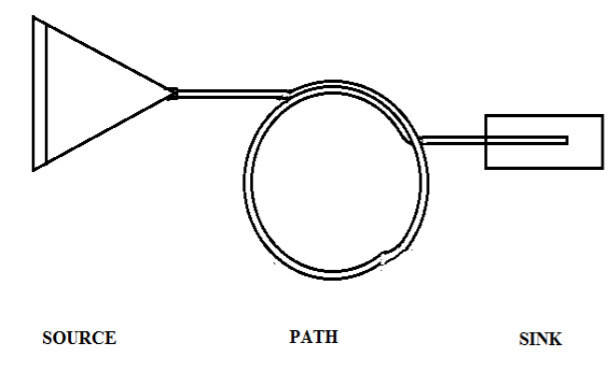
\includegraphics[height=0.4\textheight, width=0.8\textwidth]{path.png}
		\end{figure}
		\begin{itemize}
			\item<1-3> Existing setup for dispersal selection
			\item<1-3> Large outbred population of \textit{Drosophila melanogaster}
		\end{itemize}

		\column{0.5\textwidth}<2-3>
		\begin{block}{Tradeoffs against dispersal}<2-3>
			\begin{itemize}
				\item<2-3> Previous work in normal food showed largely \underline{cost-free} selection response.
				\item<3> \emph{Could costs be detected in a nutritionally-deprived context?}
			\end{itemize}
		\end{block}
	\end{columns}}
% \end{frame}

% \begin{frame}{Background}
	\only<4-6>{\begin{itemize}
		\item<4-> Dispersal evolution with the same setup, but with larval malnutrition
		\item<4-> Malnutrition $\implies$ development in food with one-third yeast concentration
	\end{itemize}

	\only<5>{\begin{block}{Selection line populations}<5>
		\begin{itemize}
			\item<5> \textbf{MD}-\underline{M}alnourished \underline{D}ispersers
			\item<5> \textbf{MC}-\underline{M}alnourished \underline{C}ontrol
		\end{itemize}
	\end{block}}

	\begin{block}{Response at generation 42}<6->
		\begin{itemize}
			\item<6-> Dispersal response seen-MD were more likely to initiate dispersal and dispersed over longer distances than MC.
			\item<6-> Locomotor activity higher in MD than in MC, but no costs in body weight or fecundity
		\end{itemize}
	\end{block}}
\end{frame}

\subsection{Post-pandemic data and future directions}
\begin{frame}{Lockdown and suspension of selection}
	\only<1-2>{\begin{itemize}
		\item<1-> Dispersal selection suspended from March to November 2020 spanning 11 generations
		\item<2-> Two assays to assess loss of phenotype before continuing selection-\emph{dry body weight and locomotor activity}
	\end{itemize}}
	\only<3>{
	\begin{block}{Locomotor activity}
		ANOVA numbers here
	\end{block}
	\begin{columns}
		\column{0.49\textwidth}
		\begin{figure}
			\centering
			\scalebox{0.35}{\input{activity.pdf_tex}}
		\end{figure}

		\column{0.49\textwidth}
		\begin{figure}
			\centering
			\scalebox{0.35}{\input{rest.pdf_tex}}
		\end{figure}
	\end{columns}}

	\only<4>{
	\begin{block}{Dry body weight}
		ANOVA numbers here
	\end{block}
	\begin{figure}
		\centering
		\scalebox{0.25}{\input{bw.pdf_tex}}
	\end{figure}}
\end{frame}
\begin{frame}{Resuming selection}
\begin{itemize}
	\item<1-> Locomotor phenotype is still detectable, body weight trends are unclear.
	\item<1-> About 20 more generations of dispersal have now been carried out-62 generations of selection in total
	\item<2-> Bigger set of assays need to be repeated-dispersal kernel, body weight and fecundity
	\item<2-> I plan to conduct smaller experiments for the time being-exploration and male-male aggression, and kit-based estimation of total glucose and triglyceride content.
	\item<3-> Standardisation-consumption rate based on coloured dye uptake and recording-based approaches to measure time to starvation or dessication
\end{itemize}
\end{frame}
\section{Cancer theory}
\subsection{Adaptive therapy}
\begin{frame}{Conventional vs adaptive therapy}
\visible<1->{\begin{figure}
	\centering
	\scalebox{0.15}{\input{comprelease.pdf_tex}}
	\caption{Drug at maximum dose-competitive release of resistant cells}
\end{figure}}
\visible<2->{\begin{figure}
	\centering
	\scalebox{0.15}{\input{at.pdf_tex}}
	\caption{Adaptive therapy and \emph{control through competition}}
\end{figure}}
\end{frame}

\begin{frame}{Ecological interactions in castration-resistant prostate cancer}
	\only<1-3>{\begin{itemize}
		\item<1-> Early prostate cancer cells-dependent on testosterone supply for growth-treated by chemical castration
		\item<2-> Some cells acquire testosterone synthesis $\implies$ castration resistance-treated with specific inhibitors
		\item<3> Other cells become testosterone-independent in growth $\implies$ resistant to inhibitors-treatment?
	\end{itemize}}
	\only<4>{\begin{block}{Three cell types and two resources}
		\begin{itemize}
			\item Oxygen-externally-supplied resource
			\item Testosterone-produced internally
			\item $T^+$-testosterone-dependent, but not producing
			\item $T^p$-testosterone-dependent, also producing as a public good
			\item $T^-$-testosterone-independent
		\end{itemize}
	\end{block}
	This work was done with Harsha, a Master's student in the lab.}
\end{frame}

\begin{frame}{A mathematical framework}
		\only<1>{
		For $i \in \{T^+,T^p,T^-\}$
		\begin{equation}
		  \frac{dy_i}{dt} = r_{i,max} y_i (1 - \frac{\sum_j y_j}{1 + K_{i,max} f_i(O_2) f_i(T)} )- \delta_i y_i
		\end{equation}

		For $R \in \{O_2,T\}$
		\begin{equation}
		  f_i(R) = \begin{cases}
		  1 &\text{if } ul_{R,i} \leq R \\
		  \frac{R-ll_{R,i}}{ul_{R,i}-ll_{R,i}} &\text{if } ll_{R,i} < R < ul_{R,i} \\
		  0 &\text{if } R \leq ll_{R,i} \\
		  \end{cases}
		\end{equation}

		\begin{equation}
		  \frac{dO_2}{dt} = p_{O_2} - \sum_i \mu_{O_2,i} y_i - \lambda_{O_2} O_2
		\end{equation}

		\begin{equation}
		  \frac{dtest}{dt} = p_{test}(abi) y_{T^p} - \sum_i \mu_{test,i} y_i - \lambda_{test} test
		\end{equation}
		}

	\only<2>{
	\begin{columns}
		\column{0.5\textwidth}
		\begin{figure}
			\centering
			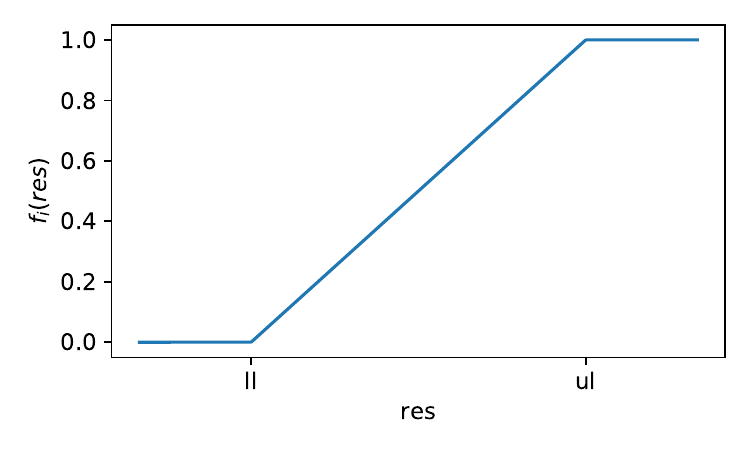
\includegraphics[width=0.8\textwidth]{f_res}
			\caption{Response function for change in carrying capacity against resource concentration}
		\end{figure}

		\column{0.5\textwidth}
		\begin{block}{Parameterisation}
			Doubling times, consumption rates for oxgen and testosterone, and testosterone production rate for $T^p$ were all derived from literature sources reporting empirical measurements in cell lines.
		\end{block}
	\end{columns}
	}
\end{frame}

\begin{frame}{Competition is tuned by resource limitation}
\visible<1-4>{\begin{figure}
		\centering
		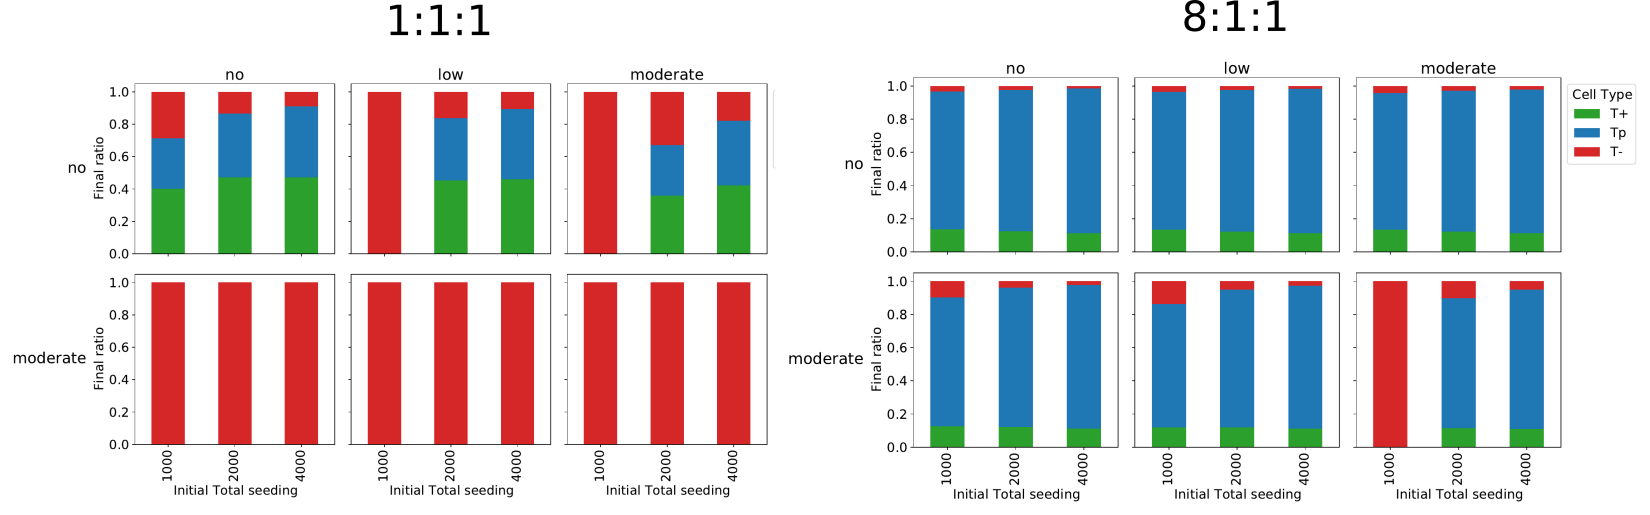
\includegraphics[width=\textwidth]{fig2}
\end{figure}}
\only<2-4>{\begin{itemize}
	\item<2-> Doubling rates scale as $T^-$<$T^+$<$T^p$, but $T^-$ doesn't win by default.
	\item<2-> Resource limitations can be used to tune co-existence.
	\item<3-> Testosterone is the stronger limiting resource in this system.
	\item<4-> Higher $T^-$ proportion makes tumours harder to treat and more unresponsive.
\end{itemize}}
\end{frame}

\begin{frame}{Further development}
	\begin{itemize}
		\item A resource-consumer model without explicit carrying capacity terms-parameterisation is ongoing
		\item Further exploration of therapy parameters in the same model-rules of on and off, frequency, multi-drug combinations
		\item Spatial dynamics-a discrete reaction-diffusion system is being considered at the moment
	\end{itemize}
	All three lines are being developed with undergraduate students from IISER Pune.
\end{frame}

\subsection{Other theory work in cancer}
\begin{frame}{Patterns in cancer incidence}
\only<1->{\begin{block}{Trends across species}
	\begin{itemize}
		\item Body size as well as lifespan varies widely across species and taxa.
		\item Cancer risk is not correlated to this variation.
	\end{itemize}
\end{block}}

\only<2->{\begin{block}{Within species-late-life decline}
	\begin{itemize}
		\item
	\end{itemize}
\end{block}}

\only<3>{\begin{block}{Timeline}

\end{block}}
\end{frame}

% \bibliographystyle{cell}
% \bibliography{review}
\begin{frame}
	\centering{\huge{Thank you for your attention.}}
\end{frame}

\end{document}
